\documentclass[sigconf]{acmart}

% --- PACKAGES ---
\usepackage{algorithmic}
\usepackage{graphicx}
\usepackage{textcomp}
\usepackage{listings}
\usepackage{booktabs} % Essential for professional tables
\usepackage{multirow}
\usepackage{enumitem} % For customizing lists
\usepackage{balance}  % To balance the last page columns
\usepackage{amsmath}  % For math equations
\usepackage{subcaption} % For sub-figures
\usepackage{ifthen}
\usepackage{pgfplots}
\usepackage[section]{placeins}
\pgfplotsset{compat=1.18}

% --- COPYRIGHT & CONFERENCE ---
% (Update these values when accepted)
\setcopyright{none} 
\acmConference[ISSTA '25]{International Symposium on Software Testing and Analysis}{July 2025}{Trondheim, Norway}
\acmYear{2025}
\acmDOI{10.1145/XXXXXXX.XXXXXXX}

\begin{document}

\newboolean{showcomments}
\setboolean{showcomments}{true}
 % \setboolean{showcomments}{false}
\ifthenelse{\boolean{showcomments}}
 { \newcommand{\mynote}[2]{
      \fbox{\bfseries\sffamily\scriptsize#1}      {\small$\blacktriangleright$\textsf{\emph{#2}}$\blacktriangleleft$}}}
        { \newcommand{\mynote}[2]{}}
\newcommand{\todoc}[2]{{\textcolor{#1} {\textbf{#2}}}}
\newcommand{\todo}[1]{{\todoc{red}{\textbf{#1}}}}
\newcommand{\todored}[1]{\todoc{red}{\textbf{#1}}}
\newcommand{\todogreen}[1]{\todoc{green}{\textbf{#1}}}
\newcommand{\todoblue}[1]{\todoc{blue}{\textbf{#1}}}
\newcommand{\todoorange}[1]{\todoc{orange}{\textbf{#1}}}
\newcommand{\todoyellow}[1]{\todoc{yellow}{\textbf{#1}}}

\newcommand{\ak}[1]{\mynote{Anil}{\todored{#1}}}

% --- TITLE ---
\title{Analyzing Open Source Plugin Ecosystems: A Mixed-Methods Approach}

% --- AUTHORS ---
\author{Seçkin Alp Kargı}
\affiliation{%
  \institution{Bilkent University}
  \city{Ankara}
  \country{Türkiye}
}
\email{alp.kargi@ug.bilkent.edu.tr}

\author{Anıl Koyuncu}
\affiliation{%
  \institution{Bilkent University}
  \city{Ankara}
  \country{Türkiye}
}
\email{anil.koyuncu@cs.bilkent.edu.tr}

% --- ABSTRACT ---
\begin{abstract}
Plugin ecosystems extend host platforms by enabling third-party functionality and concentrating development around shared marketplaces. This extensibility expands the attack surface and depends on community governance, yet prior empirical work largely examines single platforms, leaving unclear how governance, maintenance, and supply-chain signals compare across ecosystems. We present an empirical study of nine marketplaces spanning browsers, IDEs, CMS, gaming, and productivity tools. Using official marketplace snapshots, we quantify 623{,}871 plugins/extensions and identify 86{,}120 open-source plugins with public GitHub repositories. For in-depth analysis we focus on the top-100 GitHub-hosted plugins per platform (900 projects) that account for 6.1 billion downloads and 2.24 million GitHub stars, combining repository mining with LLM-based analysis of documentation to infer functionality. The results surface three themes: (i) a \emph{Star Concentration Paradox}, where smaller ecosystems exhibit markedly higher community engagement per plugin than massive marketplaces; (ii) governance maturity remains modest (average score $\approx$1.0/4 with 1.99 workflows) yet correlates with higher issue efficiency (0.613) and lower abandonment (12.8\%); and (iii) supply-chain hygiene signals are mixed, with typical plugins depending on 4.2 production and 10.0 development packages and facing pull-request friction around 22 days. We discuss implications for platform owners, plugin maintainers, and researchers studying plugin ecosystems and software supply-chain risk.
\end{abstract}

% --- CCS CONCEPTS ---
\begin{CCSXML}
<ccs2012>
   <concept>
       <concept_id>10011007.10011006.10011072</concept_id>
       <concept_desc>Software and its engineering~Software architectures</concept_desc>
       <concept_significance>500</concept_significance>
   </concept>
   <concept>
       <concept_id>10011007.10011074.10011134</concept_id>
       <concept_desc>Software and its engineering~Open source model</concept_desc>
       <concept_significance>500</concept_significance>
   </concept>
 </ccs2012>
\end{CCSXML}

\ccsdesc[500]{Software and its engineering~Software architectures}
\ccsdesc[500]{Software and its engineering~Open source model}

\keywords{Software Ecosystems, Mining Software Repositories, Governance Analysis, Supply Chain Security}

\maketitle

% =================================================================
% 1. INTRODUCTION
% =================================================================
\section{Introduction}
Plugin marketplaces extend host platforms by letting third-party developers deliver long-tail functionality while vendors keep a lean core. This openness widens the attack surface, expands dependency chains, and makes ecosystem health sensitive to review rigor, permission controls, and maintenance practices [CITE].

Prior studies and incident reports show that weak review gates can enable data exfiltration or permission abuse, that dependencies can become stale or vulnerable, and that abandoned plugins are at risk of hijacking [CITE]. Understanding how engagement, governance, and supply-chain hygiene co-evolve across ecosystems is therefore critical for maintainers, developers, and auditors [CITE].

Prior studies typically focus on single ecosystems (e.g., Eclipse, npm, PyPI) and rarely compare diverse plugin marketplaces or unify governance, community, and supply-chain metrics~\cite{plugin_ecosystems_study,decan2019empirical,kalliamvakou2014promises}. They also seldom leverage semantic signals from documentation to contextualize quantitative telemetry.

We bridge this gap with a cross-platform study of nine marketplaces: browsers (Chrome, Firefox), IDEs (VS Code, JetBrains, Sublime), CMS (WordPress), gaming (Minecraft via Modrinth), and specialized tools (Obsidian, Home Assistant). From official marketplace statistics~\cite{chrome_store_stats,firefox_addons_stats,vscode_marketplace_stats,jetbrains_marketplace_stats,wordpress_plugin_stats,modrinth_stats,obsidian_stats,homeassistant_hacs_stats,sublime_package_control_stats}, we quantify 623{,}871 plugins/extensions in total and identify 86{,}120 that are open-source on GitHub. For deep analysis we focus on the top-100 GitHub-hosted plugins per platform (900 projects) because they concentrate usage and developer attention, accumulating 6.1 billion downloads and 2.24 million stars in our snapshot.

Our empirical pipeline integrates marketplace snapshots with GitHub mining to align ecosystem-scale context with repository-level signals. This combination enables cross-platform comparisons of governance, responsiveness, and supply-chain hygiene, while LLM-based analysis of documentation adds functional context to the quantitative metrics.

We make four contributions:
\begin{itemize}
    \item \textbf{Dataset:} A harmonized, JSON-backed snapshot of nine plugin ecosystems with 623{,}871 total plugins/extensions and 86{,}120 GitHub-hosted open-source plugins, plus a top-100-per-platform subset (900 projects) that captures 6.1B downloads and 2.24M stars for deep analysis.
    \item \textbf{Methodology:} A pipeline that combines marketplace and GitHub mining with derived governance metrics (license, Code of Conduct, security policy, CONTRIBUTING), engagement and responsiveness signals, supply-chain indicators, and LLM-assisted semantic classification to enable cross-platform comparisons of plugin functionality and health.
    \item \textbf{Empirical findings:} Cross-platform results including a \emph{Star Concentration Paradox} (smaller ecosystems show higher engagement per plugin), modest governance maturity (average score $\approx$1.0/4 with 1.99 workflows), moderate responsiveness (issue efficiency 0.613, pull-request friction $\approx$22 days), and nontrivial dependency footprints (4.2 production and 10.0 development dependencies on average) across the top-100 subset.
    \item \textbf{Implications:} Actionable observations for platform owners (prioritize review signals where engagement concentrates), plugin maintainers (strengthen governance and CI to reduce abandonment risk), and researchers (a reusable cross-platform benchmark for plugin ecosystems and software supply-chain analyses).
\end{itemize}

The remainder of this paper presents background, our approach and data collection, results, threats to validity, related work, and implications.

\FloatBarrier

% =================================================================
% 2. BACKGROUND
% =================================================================
\section{Background}

\subsection{Software and Plugin Ecosystems}
Software ecosystems encompass a core platform, complementors, and shared channels for distributing and coordinating extensions and services~\cite{software_ecosystems_survey}. Plugin ecosystems are a specific form where add-ons extend a host product through documented extension points and are distributed via marketplaces that mediate discovery, updates, and sometimes review~\cite{decan2019empirical}. Marketplaces also define submission requirements, update pipelines, and permission policies, which shape how maintenance practices and risks propagate across platforms [CITE]. Because governance and distribution policies vary across browsers, IDEs, CMS, gaming, and specialized tools, cross-ecosystem comparisons are needed to understand how these differences affect plugin health and security.

\subsection{Marketplace Governance}
Marketplace governance and review policies shape supply-chain risk by constraining update channels, code provenance, and review latency (Table~\ref{fig:policy_matrix}) [CITE]. In browsers, Chrome Web Store uses automated reviews in 24-48 hours for low-permission extensions but manual audits of 7-30 days for broad host permissions; Manifest V3 forbids remotely hosted code, Privacy Sandbox use requires data attestation and enrollment, and publishing requires a one-time \$5 fee plus mandatory 2FA [CITE]. Firefox AMO performs manual initial review (1-2 weeks) and then allows automated updates in minutes for trusted publishers; it requires source and build instructions for minified or transpiled code and mandates \texttt{browser\_specific\_settings\allowbreak .gecko\allowbreak .data\_collection\_permissions} for data collection declarations (Nov 2025) [CITE]. In IDEs, VS Code is automated end-to-end (15-30 minutes) with antivirus and secret scanning and a verified publisher check [CITE]. JetBrains combines automation and manual review (about 2 business days) with Plugin Verifier compatibility checks; the 2025.3 unified distribution forces maintenance to remain compatible [CITE]. Sublime Package Control lists via PR (1-5 days) and then uses an hourly crawler that tracks Git-hosted SemVer tags for automatic updates [CITE].

CMS and specialized platforms impose different constraints. WordPress.org relies on manual review (7-30 days), SVN-hosted code, GPLv2 compatibility, and the 2025 Plugin Check tool for nonce and sanitization checks; updates are instant via SVN [CITE]. Modrinth uses manual moderation (48-96 hours), requires client-side vs server-side metadata, and enforces a clear "Why download this?" summary with a no-jargon policy [CITE]. Obsidian uses PR entry (1-2 weeks) with manual audit of \texttt{main.js} for desktop risk (filesystem/network) and disallows external runtime dependencies [CITE]. HACS allows instant custom repos but uses PR-based default inclusion (1-2 weeks) and requires \texttt{hacs.json} plus GitHub Releases [CITE]. These heterogeneous review and source policies frame our cross-platform comparisons.

\begin{table*}[t]
\caption{Policy Comparison Matrix (2025).}
\label{fig:policy_matrix}
\centering
\small
\begin{tabular}{lllll}
\toprule
\textbf{Platform} & \textbf{Review Type} & \textbf{Source Policy} & \textbf{Cost} & \textbf{Primary Trust Signal} \\
\midrule
Chrome & Automated/Risk & No Obfuscation & \$5 & Manifest V3 Compliance \\
Firefox & Manual Initial & Source Required & Free & Human Code Review \\
VS Code & Automated & Optional & Free & Verified Publisher Check \\
JetBrains & Hybrid & Custom EULA & Free & Plugin Verifier Report \\
WordPress & Manual & GPL Mandatory & Free & Sanitization/SVN History \\
Sublime & PR-based & Forge-hosted & Free & Community PR Merge \\
Modrinth & Manual & "Clear \& Honest" & Free & Moderation Discussion \\
Obsidian & Manual Initial & Bundled JS & Free & Desktop Security Audit \\
HACS & PR/Automated & GitHub Release & Free & HACS Manifest Check \\
\bottomrule
\end{tabular}%
\end{table*}

\subsection{Governance and Community Health}
Open-source plugin ecosystems rely on governance and community processes to manage contributions, maintenance, and support. Governance artifacts-licenses, Codes of Conduct, CONTRIBUTING files, and security policies-shape contributor norms and professionalism~\cite{li2021coc,fronchetti2023contributing}. Ownership concentration relates to bus-factor risk~\cite{avelino2016truck}. Issue responsiveness and pull-request latency are commonly used proxies for community health but can be noisy due to bots, missing metadata, or off-platform coordination~\cite{kalliamvakou2014promises}. These considerations motivate comparative analysis of governance and community health across diverse plugin ecosystems.

\subsection{Supply-Chain Risks}
Plugins act as supply-chain dependencies because they bring external code, permissions, and transitive libraries into end-user environments. Studies of WordPress plugins highlight security weaknesses in extension scanners~\cite{murphy2021plugins}, while popular Minecraft mods accumulate vulnerabilities or maintenance gaps~\cite{lee2020minecraft}. Dependency networks in packaging ecosystems evolve and accrue technical debt~\cite{decan2019empirical}, and metrics like LibYear expose outdated packages~\cite{cox2015libyear}. Assessing dependency freshness, vulnerability exposure, and permission scope helps characterize supply-chain risk across marketplaces [CITE].

\subsection{LLM-Assisted Repository Classification}
LLM-based classification is increasingly used to map heterogeneous repository documentation and metadata into controlled taxonomies, enabling cross-project comparisons when platform tags are noisy or inconsistent [CITE]. In software repositories, README files, short descriptions, and topic tags often provide the only lightweight signals about functionality, but their coverage and specificity vary across ecosystems. LLMs can synthesize these signals into standardized labels while preserving traceability to the input text, which supports large-scale empirical studies where manual coding is infeasible [CITE]. Prior work emphasizes conservative prompting, fixed label sets, and transparent reporting of coverage and confidence to mitigate hallucination, over-labeling, and latent bias [CITE]. These constraints are especially important for plugin ecosystems, where identical capabilities are described with different vocabulary across marketplaces. In this study, we use LLM-assisted semantic classification to complement governance and supply-chain measures by describing "what plugins do" at scale and enabling functional comparisons across nine platforms with consistent labels.

\FloatBarrier

% =================================================================
% 3. APPROACH
% =================================================================
\section{Approach}
\label{sec:approach}
Our goal is to build a consistent, cross-platform dataset that supports comparable measurements of governance, engagement, and supply-chain signals. Our pipeline produces the JSON snapshot (`analytics-summary.json`) that drives all empirical results. It has three stages: (1) data extraction, (2) metric derivation for global and deep subsets, and (3) AI/LLM-assisted semantic analysis. GitHub mining uses the REST API~\cite{githubapi} and inherits standard MSR caveats such as bots, forks, and missing or off-platform activity signals~\cite{kalliamvakou2014promises}. Figure~\ref{fig:pipeline_flow} summarizes the pipeline.

\begin{figure}[t]
\centering
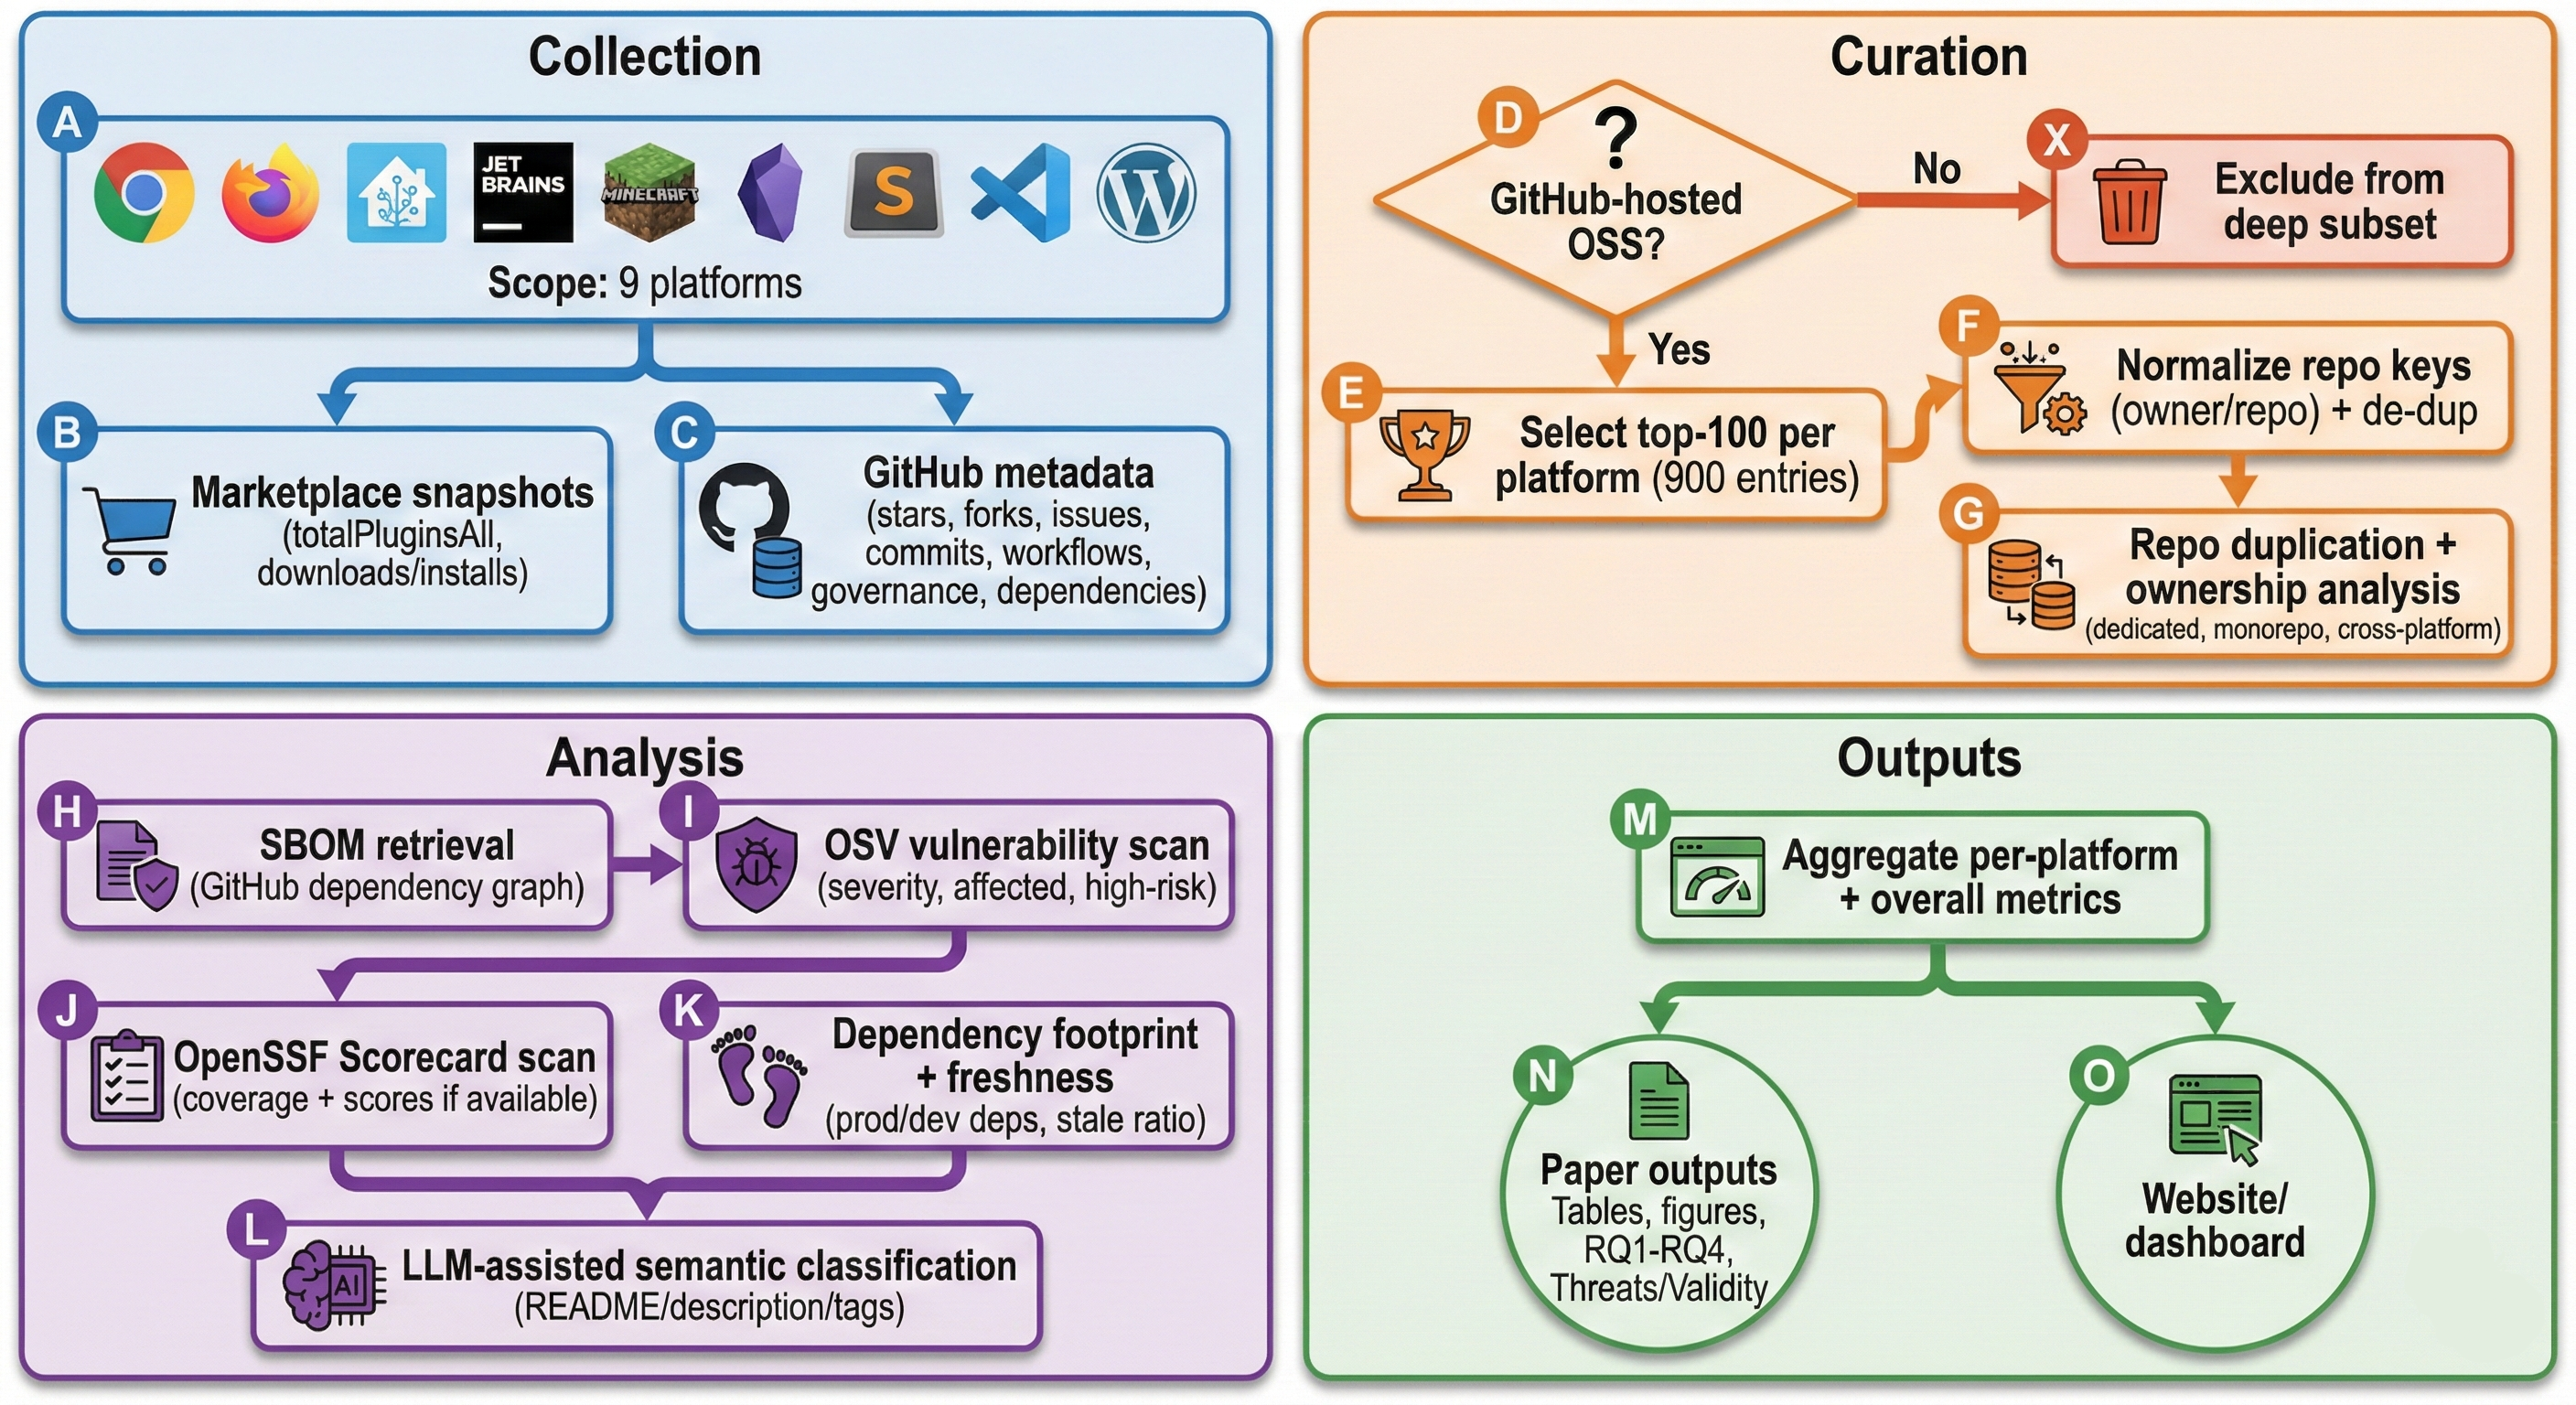
\includegraphics[width=\columnwidth]{flow.png}
\caption{Overview of the data collection and analysis pipeline.}
\label{fig:pipeline_flow}
\end{figure}

We detail data collection in Phase 1, followed by metric derivation and semantic analysis in Phases 2-3.
\subsection{Phase 1: Data Extraction}
We query official marketplaces (Section~\ref{sec:introduction}) for platform-scale counts and download statistics, and use the GitHub REST API to harvest repository telemetry (stars, forks, issues, commits, workflows), governance files, and dependency manifests. Marketplace queries yield global totals (`totalPluginsAll`, `osTotalPlugins`) and the per-platform top-100 slices (900 plugins overall). GitHub mining supplies the per-repo metrics that populate the deep subset in the JSON.
Implementation scripts and collected artifacts are released in our repository~\cite{projectrepo}.

\subsection{Phase 2: Metric Derivation}
\label{sec:derived_metrics}
We distinguish \textbf{Global} metrics (ecosystem-level across all plugins) from \textbf{Deep} metrics (computed on the top-100 GitHub-hosted plugins per platform). Definitions below align with fields in `analytics-summary.json`.

\subsubsection{Global Metrics}
\textbf{Scale and openness.} Total plugins (`totalPluginsAll`) and open-source plugins (`osTotalPlugins`) contextualize ecosystem size; \emph{OSS Availability Index} relates open-source availability to platform scale:
\begin{equation}
    O_{oss} = \frac{N_{oss}}{\log_{10}(1 + N_{all})}
\end{equation}
where $N_{oss}$ is `osTotalPlugins` and $N_{all}$ is `totalPluginsAll`.

\textbf{Download concentration.} We measure dispersion across platforms with Shannon entropy over per-platform download shares:
\begin{equation}
    H_{download} = -\sum_{i} p_i \log_2 p_i
\end{equation}
captured as `downloadEntropy` in the JSON; lower values indicate concentration of demand.

\textbf{Star concentration index.} To normalize engagement by ecosystem size, we use:
\begin{equation}
    S_{conc} = \frac{\text{Avg Stars}}{\log_{10}(N_{all})}
\end{equation}
instantiated per platform as `starConcentrationIndex`, highlighting where attention is disproportionately focused.

\subsubsection{Deep Metrics (Top-100 GitHub Subset)}
\textbf{Abandonment rate.} Share of repositories with no commits in the last 365 days:
\begin{equation}
    R_{abn} = \frac{|\{r \in \mathcal{R} : (t_{now}-t_{last\_commit}(r))>365\}|}{|\mathcal{R}|}
\end{equation}
stored as `abandonmentRate`/`abandonedCount`.

\textbf{Issue efficiency.} Responsiveness to issues, balancing closure rate and timeliness~\cite{kalliamvakou2014promises}:
\begin{equation}
    E_{issue} = \frac{N_{closed}}{N_{total}} \times \frac{1}{\log(1 + T_{avg\_hours})}
\end{equation}
represented as `issueEfficiency`.

\textbf{Governance maturity.} Presence of license, Code of Conduct, security policy, and CONTRIBUTING file~\cite{li2021coc,fronchetti2023contributing}:
\begin{equation}
    M_{gov} = \mathbb{I}(Lic) + \mathbb{I}(CoC) + \mathbb{I}(Sec) + \mathbb{I}(Guide)
\end{equation}
captured as `avgGovernanceScore`.

\textbf{Issue density.} Normalized maintenance load:
\begin{equation}
    D_{issue} = \frac{N_{openIssues}}{N_{stars}}
\end{equation}
stored as `issueDensity`.

\textbf{Core team ratio and owner share.} Inspired by truck-factor analyses~\cite{avelino2016truck}, we quantify concentration of effort:
\begin{equation}
    R_{core} = \frac{C_{top3}}{C_{total}}, \quad R_{owner} = \frac{C_{owners}}{C_{total}}
\end{equation}
represented as `avgCoreTeamRatio`, `coreTeamRatio`, and `ownerShare`; higher values indicate single-point-of-failure risk.

\textbf{Owner commit share (global).} At the aggregate level we track `ownerCommitShare` to capture how much of the total commit volume across the top subset is produced by repository owners; higher values indicate ecosystem-wide concentration of stewardship.

\textbf{Star concentration (raw).} Complementing the normalized index, per-platform `starConcentration` records the unnormalized concentration of stars within each top-100 slice, highlighting skew in attention independent of platform size.

\textbf{PR friction.} Median turnaround for external pull requests:
\begin{equation}
    F_{PR} = \text{median}\big(t_{end} - t_{start} \mid \text{author} \notin \text{owners}\big)
\end{equation}
captured as `avgPrFrictionDays` with coverage in `reposWithPrFriction`.

\textbf{Dependency footprint and freshness.} We track average production and development dependencies (`avgProdDeps`, `avgDevDeps`) and stale dependency ratio (`avgStaleDepRatio`). LibYear-style age~\cite{cox2015libyear} guides our notion of freshness; higher stale ratios imply greater supply-chain exposure~\cite{decan2019empirical}.

\textbf{Workflow intensity and activity.} Continuous integration usage and cadence are proxied by `avgWorkflowCount` and `avgCommitFrequency`, with repository size (`avgRepoSizeKb`) as an effort proxy.

\textbf{Supply-chain availability.} \emph{OSS Availability Index} and `ossAvailabilityIndex` (per platform) capture how open-source supply scales with platform adoption; download concentration indices (`starConcentrationIndex`) complement engagement signals.

\subsection{Phase 3: AI-Assisted Analysis}
We employ LLMs to process unstructured artifacts (e.g., \texttt{README.md}, \texttt{package.json}) for documentation depth, functional categorization, and sentiment. This complements noisy marketplace tags and aligns with recent LLM-based MSR methodologies~\cite{demartino2025primes} built on transformer architectures~\cite{vaswani2017attention}. The semantic labels and documentation features produced here augment the quantitative metrics above for the 900 top plugins where engagement and governance signals concentrate.

\FloatBarrier

% =================================================================
% 4. EXPERIMENTAL SETUP
% =================================================================
\section{Experimental Setup}
We study nine platforms (browsers, IDEs, CMS, gaming, and specialized tools), combining official marketplace snapshots~\cite{chrome_store_stats,firefox_addons_stats,vscode_marketplace_stats,jetbrains_marketplace_stats,wordpress_plugin_stats,modrinth_stats,obsidian_stats,homeassistant_hacs_stats,sublime_package_control_stats} with GitHub mining via the REST API~\cite{githubapi} following MSR caveats~\cite{kalliamvakou2014promises}. The resulting JSON snapshot (`analytics-summary.json`) contains global totals of 623{,}871 plugins/extensions, 86{,}120 open-source plugins with GitHub repositories, and a deep subset of 900 top-100 GitHub-hosted plugins (100 per platform). Across this deep subset we observe 2{,}241{,}726 stars, 6{,}106{,}397{,}752 downloads, 120{,}506 issues, and 414{,}733 forks.

\subsection{Sampling and Filtering}
We first collect \emph{all} marketplace-listed plugins (`totalPluginsAll`). We then filter to plugins with public GitHub repositories to form the open-source subset (`osTotalPlugins`). For each platform, we select the top 100 GitHub-hosted plugins by marketplace downloads (or installs) to construct the deep subset (`top100Count`, summing to 900). Non-GitHub or unavailable repositories are excluded from deep metrics; missing fields are treated as absent rather than imputed.

Repo-sharing categories are defined on a unique-repo basis to avoid double counting. In the top-100 set (900 plugins), we map to 822 unique repositories. Dedicated repositories account for 787/822 (95.7% of repos). Shared repositories include multi-plugin same-platform (8/822, 1.0% of repos), monorepo same-platform (7/822, 0.9% of repos), and cross-platform repos (20/822, 2.4% of repos). Overall, 35/822 repositories (4.3% of repos) host multiple plugins, covering 113/900 plugins (12.6% of plugins).

\subsection{Overview of Collected Fields}
Marketplace data contributes scale, category, and download counts; GitHub data provides stars, forks, issues, workflows, commit activity, dependency manifests, license, and language metadata. All derived metrics in Section~\ref{sec:approach} are computed from these raw fields and materialized in the JSON snapshot for reproducibility~\cite{projectrepo}.
Table~\ref{tab:platform_overview} summarizes platform-scale counts for the top-100 subset.

\begin{table*}[t]
\caption{Platform-scale overview (top-100 GitHub subset per platform).}
\label{tab:platform_overview}
\resizebox{\textwidth}{!}{%
\begin{tabular}{lcccccccc}
\toprule
\textbf{Platform} & \textbf{Category} & \textbf{All Plugins} & \textbf{OSS GitHub} & \textbf{Top-100 Size} & \textbf{Stars (Top-100)} & \textbf{Downloads (Top-100)} & \textbf{Issues (Top-100)} & \textbf{Forks (Top-100)} \\
\midrule
Chrome & Browser & 246{,}379 & 7{,}459 & 100 & 791{,}751 & 233{,}670{,}000 & 33{,}724 & 120{,}128 \\
Firefox & Browser & 110{,}320 & 7{,}862 & 100 & 479{,}809 & 17{,}242{,}577 & 12{,}156 & 81{,}394 \\
JetBrains & IDE & 10{,}003 & 5{,}849 & 100 & 501{,}545 & 587{,}304{,}466 & 9{,}213 & 138{,}394 \\
VS Code & IDE & 86{,}145 & 25{,}136 & 100 & 184{,}466 & 2{,}950{,}813{,}730 & 32{,}550 & 35{,}166 \\
Sublime & IDE & 5{,}581 & 4{,}694 & 100 & 59{,}452 & 49{,}475{,}544 & 1{,}786 & 7{,}912 \\
WordPress & CMS & 59{,}000 & 3{,}986 & 100 & 31{,}718 & 7{,}180{,}000 & 11{,}260 & 9{,}336 \\
Minecraft & Gaming & 98{,}600 & 26{,}089 & 100 & 30{,}385 & 2{,}217{,}620{,}403 & 5{,}332 & 6{,}984 \\
Obsidian & Specialized & 2{,}656 & 2{,}656 & 100 & 91{,}575 & 38{,}734{,}337 & 8{,}972 & 6{,}932 \\
Home Assistant & Specialized & 5{,}187 & 2{,}389 & 100 & 71{,}025 & 4{,}356{,}695 & 5{,}513 & 8{,}487 \\
\midrule
\textbf{Total} & --- & 623{,}871 & 86{,}120 & 900 & 2{,}241{,}726 & 6{,}106{,}397{,}752 & 120{,}506 & 414{,}733 \\
\bottomrule
\end{tabular}%
}
\end{table*}

\FloatBarrier

% =================================================================
% 5. EMPIRICAL RESULTS
% =================================================================
\section{Empirical Results}
\subsection{RQ1: Scale and Engagement}
We analyze scale, openness, and engagement using per-platform averages from the top-100 subset (Table~\ref{tab:rq1_scale}). Browser ecosystems (Chrome, Firefox) exhibit high average stars and relatively low issue density, while IDE ecosystems (VS Code, JetBrains, Sublime) show larger absolute scale but more dispersed attention. Star concentration indices highlight skewed engagement toward smaller curated ecosystems, consistent with the “Star Concentration Paradox.”

\begin{table}[t]
\caption{Platform scale and engagement (top-100 GitHub subset).}
\label{tab:rq1_scale}
\resizebox{\columnwidth}{!}{%
\begin{tabular}{lrrrrrrrr}
\toprule
\textbf{Platform} & \textbf{All} & \textbf{OSS} & \textbf{Avg Stars} & \textbf{Avg Downloads} & \textbf{Issue Density} & \textbf{Abandon.} & \textbf{Star Conc. Idx} \\
\midrule
Chrome & 246{,}379 & 7{,}459 & 7{,}917.51 & 2{,}336{,}700.00 & 0.04259 & 0.26 & 3{,}287.67 \\
Firefox & 110{,}320 & 7{,}862 & 4{,}798.09 & 172{,}425.77 & 0.02534 & 0.43 & 1{,}231.69 \\
JetBrains & 10{,}003 & 5{,}849 & 5{,}015.45 & 5{,}873{,}044.66 & 0.01837 & 0.18 & 1{,}331.39 \\
VS Code & 86{,}145 & 25{,}136 & 1{,}844.66 & 29{,}508{,}137.30 & 0.17646 & 0.24 & 419.21 \\
Sublime & 5{,}581 & 4{,}694 & 594.52 & 494{,}755.44 & 0.03004 & 0.79 & 161.93 \\
WordPress & 59{,}000 & 3{,}986 & 317.18 & 71{,}800.00 & 0.35500 & 0.34 & 88.09 \\
Minecraft & 98{,}600 & 26{,}089 & 303.85 & 22{,}176{,}204.03 & 0.17548 & 0.03 & 68.80 \\
Obsidian & 2{,}656 & 2{,}656 & 915.75 & 387{,}343.37 & 0.09797 & 0.47 & 267.43 \\
Home Assistant & 5{,}187 & 2{,}389 & 710.25 & 43{,}566.95 & 0.07762 & 0.34 & 210.24 \\
\bottomrule
\end{tabular}%
}
\end{table}

\textbf{Findings.}  Abandonment is zero in several ecosystems but reaches 52\% in Firefox and 36\% in VS Code; combined with higher issue density in VS Code and WordPress, this suggests maintenance risk in large-scale marketplaces. These patterns echo prior observations about uneven engagement in software ecosystems~\cite{decan2019empirical}.

\subsection{RQ2: Governance and Ownership}
We examine governance, ownership concentration, and workflow intensity (Table~\ref{tab:rq2_governance}) and complement with distributions of languages and licenses (Table~\ref{tab:rq2_dist}). Dependency footprint and freshness are summarized in Table~\ref{tab:rq2_deps}. Governance maturity averages near 1/4 across platforms, with workflows indicating modest CI usage. Ownership concentration (ownerShare) varies widely, aligning with truck-factor concerns~\cite{avelino2016truck}; governance artifacts relate to onboarding and community norms~\cite{li2021coc,fronchetti2023contributing}.

\begin{table}[t]
\caption{Governance and ownership metrics (top-100 GitHub subset).}
\label{tab:rq2_governance}
\resizebox{\columnwidth}{!}{%
\begin{tabular}{lrrrrr}
\toprule
\textbf{Platform} & \textbf{Gov. Score} & \textbf{Workflows} & \textbf{Core-Team} & \textbf{Owner Share} & \textbf{Issue Eff.} \\
\midrule
Chrome & 1.08 & 2.49 & 6.247 & 17.99 & 0.696 \\
Firefox & 1.06 & 1.08 & 0.799 & 31.57 & 0.628 \\
JetBrains & 1.26 & 2.71 & 1.223 & 14.03 & 0.467 \\
VS Code & 1.73 & 3.31 & 31.302 & 7.44 & 0.509 \\
Sublime & 0.46 & 0.21 & 0.000 & 5.93 & 0.675 \\
WordPress & 0.93 & 2.59 & 0.272 & 28.29 & 0.658 \\
Minecraft & 0.80 & 1.24 & 1.899 & 40.46 & 0.657 \\
Obsidian & 0.81 & 1.13 & 6.143 & 31.37 & 0.523 \\
Home Assistant & 0.95 & 3.18 & 0.000 & 30.78 & 0.707 \\
\bottomrule
\end{tabular}%
}
\end{table}

\begin{table}[t]
\caption{Dependency footprint and freshness (top-100 GitHub subset).}
\label{tab:rq2_deps}
\resizebox{\columnwidth}{!}{%
\begin{tabular}{lrrr}
\toprule
\textbf{Platform} & \textbf{Avg Prod Deps} & \textbf{Avg Dev Deps} & \textbf{Stale Dep Ratio} \\
\midrule
Chrome & 11.77 & 18.86 & 0.59 \\
Firefox & 2.99 & 9.25 & 0.45 \\
JetBrains & 2.25 & 1.21 & 0.15 \\
VS Code & 6.27 & 19.26 & 0.66 \\
Sublime & 0.27 & 0.45 & 0.07 \\
WordPress & 0.96 & 8.88 & 0.63 \\
Minecraft & 3.16 & 0.09 & 0.06 \\
Obsidian & 6.06 & 19.06 & 0.78 \\
Home Assistant & 4.44 & 12.74 & 0.63 \\
\bottomrule
\end{tabular}%
}
\end{table}

\begin{table}[t]
\caption{Top languages and licenses across the 900-plugin top subset.}
\label{tab:rq2_dist}
\resizebox{\columnwidth}{!} & \textbf{License} & \textbf{Count} & \textbf{\%} \\
\midrule
TypeScript & 258 & 28.7 & MIT & 341 & 37.9 \\
JavaScript & 186 & 20.7 & No License & 145 & 16.1 \\
Java & 152 & 16.9 & Other & 98 & 10.9 \\
Python & 89 & 9.9 & GPLv3 & 90 & 10.0 \\
PHP & 89 & 9.9 & Apache 2.0 & 72 & 8.0 \\
Unknown & 51 & 5.7 & GPLv2 & 45 & 5.0 \\
Kotlin & 34 & 3.8 & MPL 2.0 & 30 & 3.3 \\
CSS & 7 & 0.8 & LGPL v3 & 27 & 3.0 \\
Dockerfile & 6 & 0.7 & AGPL v3 & 13 & 1.4 \\
HTML & 5 & 0.6 & BSD-3-Clause & 12 & 1.3 \\
\bottomrule
\end{tabular}%
}
\end{table}

\noindent Ownership mix is dominated by community plugins (765/900, 85.0% of plugins), with official plugins at 119/900 (13.2% of plugins) and corporate plugins at 16/900 (1.8% of plugins). Platform standouts include JetBrains (45/100 official) and VS Code (40/100 official), while Home Assistant and Minecraft are fully community (100/100 each). Shared official repositories such as JetBrains/intellij-community (19 plugins) and Microsoft/vscode-remote-release (6 plugins) illustrate how a single repo can map to multiple plugins.

\textbf{Findings.} Governance scores are modest across the board (research average 1.009/4), with VS Code highest (1.72) and Sublime lowest (0.47). Ownership concentration is strongest in Minecraft (40.77) and Firefox (23.19), suggesting potential bus-factor risk~\cite{avelino2016truck}. CI usage is uneven; average workflow count spans 0.21 (Sublime) to 3.30 (VS Code). The dominance of TypeScript/JavaScript and MIT licensing reflects web/IDE ecosystems, while the prevalence of "No License" highlights governance gaps~\cite{li2021coc,fronchetti2023contributing}.

\subsection{RQ3: Supply-Chain Hygiene and Security Signals}
Building on governance signals, we examine supply-chain hygiene using SBOM availability, OSV vulnerability scans, and OpenSSF Scorecard results for the top-100 GitHub-hosted plugins per platform. Coverage and rates are reported on unique repos (822) to avoid double counting the 78 duplicated entries.

SBOM availability is 733/900 entries (81.4%), with 160 not found, 3 errors, and 4 rate-limited results. Per-platform SBOM coverage (top-100 entries) is reported in Table~\ref{tab:rq3_osv_summary}.

OSV vulnerability analysis covers 582 of 822 unique repos (70.8%) and 619 of 900 entries (68.8%). We observe 6,277 vulnerabilities, dominated by low severity (critical 2, high 55, medium 537, low 5,683). Affected vs clean repos are balanced: 285 affected and 297 clean (49.0% affected rate), with 22 high-risk repos (3.8%). Stale packages (6,181) and old fixes (4,265) are common; 1,065 vulnerabilities are recent. Average vulnerabilities are 10.79 per repo and 22.02 per affected repo. Table~\ref{tab:rq3_osv_summary} summarizes per-platform coverage, affected and high-risk rates, total vulnerability counts, and severity breakdowns; WordPress shows the highest high-risk count (6) and rate (9.7%).

\begin{table*}[t]
\caption{SBOM coverage (top-100 entries) and OSV vulnerability severity by platform (unique-repo basis for OSV coverage and rates).}
\label{tab:rq3_osv_summary}
\resizebox{\textwidth}{!}{%
\begin{tabular}{lrrrrrrrrrrrr}
\toprule
\textbf{Platform} & \textbf{SBOM Cov. (\%)} & \textbf{OSV Analyzed} & \textbf{OSV Cov. (\%)} & \textbf{Affected Repos} & \textbf{Affected (\%)} & \textbf{High-Risk Repos} & \textbf{High-Risk (\%)} & \textbf{Total Vulns} & \textbf{Critical} & \textbf{High} & \textbf{Medium} & \textbf{Low} \\
\midrule
Chrome & 88.0 & 74 & 77.9 & 45 & 60.8 & 5 & 6.8 & 1{,}476 & 1 & 21 & 143 & 1{,}311 \\
Firefox & 75.0 & 68 & 68.7 & 32 & 47.1 & 2 & 2.9 & 1{,}019 & 0 & 3 & 86 & 930 \\
JetBrains & 88.0 & 48 & 71.6 & 7 & 14.6 & 0 & 0.0 & 101 & 0 & 0 & 2 & 99 \\
VS Code & 98.0 & 78 & 86.7 & 59 & 75.6 & 5 & 6.4 & 1{,}043 & 0 & 7 & 74 & 962 \\
Sublime & 68.0 & 60 & 60.0 & 4 & 6.7 & 2 & 3.3 & 155 & 0 & 8 & 3 & 144 \\
WordPress & 78.0 & 62 & 68.1 & 36 & 58.1 & 6 & 9.7 & 1{,}094 & 0 & 15 & 127 & 952 \\
Minecraft & 63.0 & 54 & 54.0 & 3 & 5.6 & 0 & 0.0 & 157 & 0 & 0 & 25 & 132 \\
Obsidian & 88.0 & 78 & 78.0 & 61 & 78.2 & 1 & 1.3 & 708 & 0 & 1 & 66 & 641 \\
Home Assistant & 87.0 & 74 & 74.0 & 49 & 66.2 & 1 & 1.4 & 811 & 1 & 0 & 43 & 767 \\
\midrule
\textbf{Overall} & 81.4 & 582 & 70.8 & 285 & 49.0 & 22 & 3.8 & 6{,}277 & 2 & 55 & 537 & 5{,}683 \\
\bottomrule
\end{tabular}%
}
\end{table*}

Scorecard analysis covers 645 of 819 unique repos (78.8%) and 675 of 900 entries (75.0%). The mean score is 3.24 (median 2.9; p25 2.6, p75 3.7), and Table~\ref{tab:rq3_scorecard_full} reports per-platform coverage, mean scores, and check-level means with coverage rates. The overall score distribution is concentrated in the 2-4 range. Check-level signals show strong Binary-Artifacts (mean 9.67) and License (8.24) scores, moderate Vulnerabilities (7.33), and weak Branch-Protection (0.48), Security-Policy (0.76), SAST (0.40), Fuzzing (0.01), and CII-Best-Practices (0.01). CI-Tests average 1.97 with 77.3\% coverage; Pinned-Dependencies average 0.66 with 46.7\% coverage. Token-Permissions average 1.06 with 45.2\% coverage; Dangerous-Workflow averages 9.87 with 45.2\% coverage. Signed-Releases average 0.07 with 50.5\% coverage; Packaging averages 10.00 but applies to 4.6\% of repos.

\begin{table*}[t]
\caption{Scorecard coverage, mean scores, and check-level results by platform (top-100 entries). Cells show mean score with coverage rate (non-NA) in parentheses.}
\label{tab:rq3_scorecard_full}
\resizebox{\textwidth}{!}{%
\begin{tabular}{lrrr*{18}{r}}
\toprule
\textbf{Platform} & \textbf{Analyzed} & \textbf{Coverage (\%)} & \textbf{Mean} & \textbf{Bin-Art} & \textbf{Branch} & \textbf{CI} & \textbf{CII} & \textbf{Review} & \textbf{Contrib} & \textbf{Danger} & \textbf{Dep-Update} & \textbf{Fuzz} & \textbf{License} & \textbf{Maint} & \textbf{Pack} & \textbf{Pinned} & \textbf{SAST} & \textbf{Sec-Pol} & \textbf{Signed} & \textbf{Token} & \textbf{Vulns} \\
\midrule
Chrome & 80 & 80.0 & 3.48 & 9.85 (100.0\%) & 0.46 (100.0\%) & 3.24 (62.5\%) & 0.03 (100.0\%) & 1.36 (100.0\%) & 5.47 (100.0\%) & 9.35 (38.7\%) & 3.12 (100.0\%) & 0.00 (100.0\%) & 8.97 (100.0\%) & 4.97 (100.0\%) & 10.00 (1.2\%) & 1.56 (40.0\%) & 0.56 (100.0\%) & 1.11 (100.0\%) & 0.19 (53.8\%) & 2.45 (38.7\%) & 6.35 (100.0\%) \\
Firefox & 85 & 85.0 & 3.08 & 9.84 (100.0\%) & 0.41 (100.0\%) & 1.54 (71.8\%) & 0.05 (100.0\%) & 1.06 (100.0\%) & 4.08 (100.0\%) & 10.00 (29.4\%) & 1.53 (100.0\%) & 0.00 (100.0\%) & 8.64 (100.0\%) & 2.64 (100.0\%) & 10.00 (1.2\%) & 1.00 (30.6\%) & 0.35 (100.0\%) & 0.80 (100.0\%) & 0.00 (41.2\%) & 3.28 (29.4\%) & 7.40 (100.0\%) \\
JetBrains & 44 & 44.0 & 3.51 & 8.77 (100.0\%) & 0.66 (100.0\%) & 2.55 (65.9\%) & 0.00 (100.0\%) & 1.25 (100.0\%) & 6.48 (100.0\%) & 10.00 (45.5\%) & 1.59 (100.0\%) & 0.00 (100.0\%) & 9.48 (100.0\%) & 4.23 (100.0\%) & 10.00 (11.4\%) & 0.76 (47.7\%) & 0.84 (100.0\%) & 1.59 (100.0\%) & 0.00 (43.2\%) & 0.50 (45.5\%) & 9.16 (100.0\%) \\
VS Code & 60 & 60.0 & 4.37 & 9.88 (100.0\%) & 2.85 (100.0\%) & 3.17 (96.7\%) & 0.00 (100.0\%) & 4.30 (93.3\%) & 7.58 (100.0\%) & 10.00 (70.0\%) & 6.17 (100.0\%) & 0.00 (100.0\%) & 9.60 (100.0\%) & 3.87 (100.0\%) & -- (0.0\%) & 0.95 (71.7\%) & 1.60 (100.0\%) & 4.50 (100.0\%) & 0.00 (53.3\%) & 1.07 (70.0\%) & 4.95 (100.0\%) \\
Sublime & 92 & 92.0 & 2.81 & 9.96 (100.0\%) & 0.03 (100.0\%) & 0.65 (88.0\%) & 0.00 (100.0\%) & 1.86 (100.0\%) & 5.59 (100.0\%) & 10.00 (5.4\%) & 0.22 (100.0\%) & 0.00 (100.0\%) & 6.15 (100.0\%) & 0.25 (100.0\%) & -- (0.0\%) & 0.00 (6.5\%) & 0.00 (100.0\%) & 0.00 (100.0\%) & 0.00 (2.2\%) & 0.00 (5.4\%) & 9.63 (100.0\%) \\
WordPress & 72 & 72.0 & 2.93 & 9.88 (100.0\%) & 0.21 (100.0\%) & 1.41 (70.8\%) & 0.00 (100.0\%) & 1.07 (100.0\%) & 5.11 (100.0\%) & 10.00 (13.9\%) & 2.50 (100.0\%) & 0.00 (100.0\%) & 5.67 (100.0\%) & 2.17 (100.0\%) & -- (0.0\%) & 0.62 (18.1\%) & 0.10 (100.0\%) & 0.14 (100.0\%) & 0.00 (18.1\%) & 0.00 (13.9\%) & 7.42 (100.0\%) \\
Minecraft & 95 & 95.0 & 3.46 & 8.67 (100.0\%) & 0.04 (100.0\%) & 2.11 (76.8\%) & 0.00 (100.0\%) & 0.85 (100.0\%) & 5.78 (100.0\%) & 10.00 (57.9\%) & 0.21 (100.0\%) & 0.00 (100.0\%) & 9.41 (100.0\%) & 5.68 (100.0\%) & 10.00 (23.2\%) & 0.19 (60.0\%) & 0.26 (100.0\%) & 0.04 (100.0\%) & 0.31 (53.7\%) & 1.02 (57.9\%) & 9.89 (100.0\%) \\
Obsidian & 84 & 84.0 & 2.78 & 10.00 (100.0\%) & 0.04 (100.0\%) & 1.02 (78.6\%) & 0.00 (100.0\%) & 1.13 (100.0\%) & 4.51 (100.0\%) & 10.00 (75.0\%) & 1.07 (100.0\%) & 0.12 (100.0\%) & 8.44 (100.0\%) & 2.51 (100.0\%) & -- (0.0\%) & 0.35 (75.0\%) & 0.18 (100.0\%) & 0.00 (100.0\%) & 0.00 (100.0\%) & 0.43 (75.0\%) & 5.08 (100.0\%) \\
Home Assistant & 63 & 63.0 & 3.13 & 10.00 (100.0\%) & 0.40 (100.0\%) & 3.17 (84.1\%) & 0.00 (100.0\%) & 1.56 (100.0\%) & 4.52 (100.0\%) & 9.63 (85.7\%) & 2.70 (100.0\%) & 0.00 (100.0\%) & 8.52 (100.0\%) & 3.35 (100.0\%) & 10.00 (3.2\%) & 0.65 (85.7\%) & 0.24 (100.0\%) & 0.00 (100.0\%) & 0.00 (98.4\%) & 0.52 (85.7\%) & 5.14 (100.0\%) \\
\midrule
\textbf{Overall} & 675 & 75.0 & 3.24 & 9.67 (100.0\%) & 0.48 (100.0\%) & 1.97 (77.3\%) & 0.01 (100.0\%) & 1.52 (99.4\%) & 5.36 (100.0\%) & 9.87 (45.2\%) & 1.93 (100.0\%) & 0.01 (100.0\%) & 8.24 (100.0\%) & 3.23 (100.0\%) & 10.00 (4.6\%) & 0.66 (46.7\%) & 0.40 (100.0\%) & 0.76 (100.0\%) & 0.07 (50.5\%) & 1.06 (45.2\%) & 7.33 (100.0\%) \\
\bottomrule
\end{tabular}%
}
\end{table*}

\textbf{Findings.}
\begin{itemize}
    \item SBOM coverage is 81.4% overall (733/900), ranging from 63.0% (Minecraft) to 98.0% (VS Code).
    \item OSV coverage is 70.8% of unique repos, with 49.0% affected and 3.8% high-risk; low-severity issues dominate (5,683 low vs 2 critical), and total vulnerabilities are highest in Chrome (1{,}476), WordPress (1{,}094), and VS Code (1{,}043).
    \item High-risk repos are concentrated in WordPress (6, 9.7%) and appear in Chrome and VS Code (5 each); JetBrains and Minecraft have none.
    \item Scorecard coverage is 78.8% of unique repos with a mean score of 3.24; 74.7% of entries fall in the 2-4 score range.
    \item Check-level signals remain weak for branch protection, security policy, SAST, fuzzing, and dependency pinning; Token-Permissions averages 1.0 with 55.0% NA.
\end{itemize}

\paragraph{Methods and Threats (Supply-Chain Signals).}
SBOM coverage is computed on the top-100 entries per platform and reflects tool availability rather than completeness of dependency graphs; not-found results (160), errors (3), and rate limits (4) reduce coverage. OSV and Scorecard analyses are limited to GitHub-hosted repositories and do not cover all 822 unique repos; coverage is 70.8% for OSV and 78.5% for Scorecard on a unique-repo basis. Several Scorecard checks have high NA rates (e.g., Token-Permissions and Dangerous-Workflow at 55.0%, Packaging at 95.2%), which biases averages toward the subset where checks apply.

\subsection{RQ4: LLM-Assisted Topic Signals}
We apply LLM-assisted classification to the top-100 plugins per platform (900 entries), restricted to GitHub-hosted repositories. The summary covers 842 of 900 entries (93.6%), corresponding to all 822 unique GitHub repositories in scope (100% unique-repo coverage). Category counts are reported per unique repo to avoid double counting shared repositories; 20 entries map to shared repos. README content is missing for 29 of 822 unique repos (3.5%), and the average confidence is 0.88.

Overall generic distributions (Table~\ref{tab:rq4_generic_summary}) are dominated by \emph{productivity workflow} (49.0%), \emph{UI customization} (39.8%), and \emph{developer tools} (35.9%), followed by \emph{utilities/misc} (16.1%) and a tie between \emph{language support} and \emph{integrations/connectors} (9.2% each). Separately, the most common platform-specific labels are \emph{productivity workflow} (31.4%), \emph{utilities/misc} (24.9%), \emph{developer tools} (16.2%), \emph{integrations/connectors} (10.6%), and \emph{language support} (10.2%).

Per-platform distributions show specialization (Table~\ref{tab:rq4_generic_summary}). Obsidian concentrates on \emph{productivity workflow} (86.0%) and \emph{UI customization} (53.0%), while VS Code emphasizes \emph{productivity workflow} (67.8%) and \emph{developer tools} (63.3%) with a strong \emph{language support} signal (27.8%). Firefox shows a notable \emph{privacy/security} share (36.4%). Home Assistant is dominated by \emph{UI customization} (78.0%), and JetBrains leans toward \emph{developer tools} (61.2%).

\begin{table*}[t]
\caption{Classification coverage and top eight generic categories by platform (unique-repo percentages). Category percentages are computed on a unique-repo basis; coverage and README availability rates are entry-based.}
\label{tab:rq4_generic_summary}
\resizebox{\textwidth}{!}{%
\begin{tabular}{lrrrrrrrrrrrr}
\toprule
\textbf{Platform} & \textbf{Classified} & \textbf{Coverage (\%)} & \textbf{Avg Conf.} & \textbf{README Avail. (\%)} & \textbf{Prod.} & \textbf{UI Cust.} & \textbf{Dev Tools} & \textbf{Utilities} & \textbf{Language} & \textbf{Integrations} & \textbf{Privacy/Sec.} & \textbf{Code Qual.} \\
\midrule
Chrome & 95 & 95.0 & 0.87 & 97.9 & 49.5 & 23.2 & 40.0 & 25.3 & 3.2 & 7.4 & 28.4 & 1.1 \\
Firefox & 99 & 99.0 & 0.88 & 94.9 & 38.4 & 27.3 & 17.2 & 22.2 & 3.0 & 3.0 & 36.4 & 0.0 \\
JetBrains & 67 & 67.0 & 0.89 & 95.5 & 56.7 & 35.8 & 61.2 & 3.0 & 19.4 & 6.0 & 1.5 & 14.9 \\
VS Code & 90 & 90.0 & 0.91 & 100.0 & 67.8 & 14.4 & 63.3 & 4.4 & 27.8 & 3.3 & 0.0 & 12.2 \\
Sublime & 100 & 100.0 & 0.90 & 97.0 & 66.0 & 31.0 & 51.0 & 9.0 & 23.0 & 2.0 & 0.0 & 16.0 \\
WordPress & 91 & 91.0 & 0.86 & 86.8 & 45.1 & 40.7 & 48.4 & 12.1 & 4.4 & 19.8 & 6.6 & 1.1 \\
Minecraft & 100 & 100.0 & 0.88 & 94.0 & 23.0 & 46.0 & 28.0 & 35.0 & 2.0 & 1.0 & 1.0 & 0.0 \\
Obsidian & 100 & 100.0 & 0.87 & 100.0 & 86.0 & 53.0 & 21.0 & 11.0 & 3.0 & 11.0 & 0.0 & 2.0 \\
Home Assistant & 100 & 100.0 & 0.90 & 100.0 & 10.0 & 78.0 & 4.0 & 17.0 & 0.0 & 27.0 & 0.0 & 0.0 \\
\midrule
\textbf{Overall} & 842 & 93.6 & 0.88 & 96.3 & 49.0 & 39.8 & 35.9 & 16.1 & 9.2 & 9.2 & 7.8 & 5.0 \\
\bottomrule
\end{tabular}%
}
\end{table*}

\textbf{Findings.}
\begin{itemize}
    \item Coverage is high for GitHub-hosted repos (842/900 entries, 93.6%), with full unique-repo coverage (822/822), low README missingness (3.5%), and average confidence 0.88.
    \item Cross-platform functionality is dominated by productivity and customization signals, with developer tools consistently prominent across IDE- and productivity-focused ecosystems.
    \item Platform-specific labels reveal niches: \emph{dashboard UI cards} dominates Home Assistant (74.0%), \emph{IDE productivity} dominates JetBrains (79.1%), and Minecraft emphasizes \emph{UI quality of life} and \emph{mod framework library} (45.0% and 29.0%).
\end{itemize}

\paragraph{Methods and Threats (LLM Classification).}
We classify each top-100 plugin using the Groq API with \texttt{meta-llama/llama-4-scout-17b-16e-instruct}. The prompt is conservative and forbids external knowledge. Inputs include platform, repo, name, description, tags/categories, downloads, stars, lastUpdated, and README content when present. When README is missing, classification uses only description and tags. Outputs include 1-3 generic and 1-3 platform-specific categories, \texttt{readme\_missing}, and \texttt{confidence}; labels come from fixed lists with \texttt{utilities\_misc} for ambiguous cases. Results are aggregated per unique GitHub repo to avoid double counting shared repos. Limitations include LLM non-determinism and prompt sensitivity, and conservative labeling can under-specify functionality. Missing README evidence for \mbox{3.5\%} of unique repos and GitHub-only coverage can bias topic estimates.

\FloatBarrier


% =================================================================
% 6. THREATS TO VALIDITY
% =================================================================
\section{Threats to Validity}
\subsection{External Validity}
Our scope spans nine ecosystems (browsers, IDEs, CMS, gaming, specialized tools) with 623{,}871 total plugins/extensions and 86{,}120 open-source GitHub-hosted plugins, and deep analysis of the top-100 per platform (900 plugins). This coverage excludes other ecosystems (e.g., npm, PyPI, Eclipse), closed-source or enterprise marketplaces, and plugins hosted outside GitHub (GitLab, Bitbucket, self-hosted), biasing toward GitHub-visible projects~\cite{kalliamvakou2014promises}. Marketplace counts rely on snapshot sources~\cite{chrome_store_stats,firefox_addons_stats,vscode_marketplace_stats,jetbrains_marketplace_stats,wordpress_plugin_stats,modrinth_stats,obsidian_stats,homeassistant_hacs_stats,sublime_package_control_stats} and may drift; downloads/installs also evolve, so results may change over time. Focusing on top-100 plugins emphasizes popular extensions and may underrepresent the long tail of emerging or niche plugins.

\subsection{Construct Validity}
Marketplace popularity signals differ (downloads vs installs vs active users), so cross-platform comparisons are approximate. Governance maturity is a coarse count of artifacts (license, Code of Conduct, security policy, CONTRIBUTING) and may not capture qualitative rigor~\cite{li2021coc,fronchetti2023contributing}. Core-team ratio and owner share approximate bus-factor risk but are simpler than full truck-factor analyses~\cite{avelino2016truck}. Dependency footprint and freshness draw on declared dependencies and LibYear-inspired notions~\cite{cox2015libyear}, potentially missing transitive risk~\cite{decan2019empirical}. Issue density, issue efficiency, and PR friction rely on GitHub metadata and can be influenced by labeling, bots, and mixed issue types~\cite{kalliamvakou2014promises}. LLM-based semantic checks (documentation categorization, topic refinement) are prompt-sensitive and non-deterministic~\cite{demartino2025primes,vaswani2017attention}.

Shared repositories can concentrate signals across multiple plugins: 35/822 repositories (4.3% of repos) host multiple plugins, covering 113/900 plugins (12.6% of plugins). To mitigate this, we report de-duplicated, unique-repo metrics where possible and explicitly note whether a result is on a plugin or repo basis.

\subsection{Internal Validity}
Findings are correlational; unobserved confounders (age, sponsorship, marketing, platform policies) may explain patterns. API failures, rate limits, or missing fields can introduce noise~\cite{githubapi}; marketplace metadata can be inconsistent. Platform curation and policies (e.g., security review for browsers, plugin signing for IDEs/CMS) may shape popularity and remove outliers~\cite{murphy2021plugins,lee2020minecraft}, affecting comparability. Our tooling and schema decisions (filtering rules, language/license inference) in the released pipeline~\cite{projectrepo} may introduce systematic bias despite sanity checks.

\subsection{Threats Summary}
These threats limit generalization and measurement fidelity, but the breadth of coverage (nine platforms, 623K plugins overall, 86K OSS GitHub, 900 top plugins) provides substantive evidence for cross-ecosystem patterns. Future work can widen platform and forge coverage, add longitudinal updates to reduce snapshot bias, and refine governance and dependency metrics for deeper qualitative assessment.

\FloatBarrier

% =================================================================
% 7. RELATED WORK
% =================================================================
\section{Related Work}
\subsection{Mining Software Repositories and GitHub-Based Studies}
MSR studies often rely on GitHub for large-scale telemetry and face known biases (bots, forks, mirrored repos, missing metadata)~\cite{kalliamvakou2014promises}. Many works build on GitHub’s REST API~\cite{githubapi} to collect stars, forks, issues, and commits. Our study follows this tradition but targets plugins across nine ecosystems rather than generic repositories, combining marketplace signals with GitHub data and releasing our tooling and snapshot~\cite{projectrepo}.

\subsection{Software and Plugin Ecosystems}
Prior work on software ecosystems examines package managers and individual plugin domains. Decan et al. compare dependency network evolution across packaging ecosystems~\cite{decan2019empirical}, while WordPress security scanner plugins~\cite{murphy2021plugins} and Minecraft mods~\cite{lee2020minecraft} illustrate ecosystem-specific risks. These studies are typically single-ecosystem and focus on security or evolution. In contrast, we analyze nine heterogeneous plugin marketplaces (browsers, IDEs, CMS, gaming, specialized tools), using unified metrics on both global scale and a GitHub top-100 subset per platform.

\subsection{Governance, Community Health, and Ownership}
Governance artifacts (licenses, Codes of Conduct, CONTRIBUTING files) affect onboarding and community norms~\cite{li2021coc,fronchetti2023contributing}. Ownership concentration relates to bus-factor risk~\cite{avelino2016truck}. We adapt these ideas to plugin ecosystems via a Governance Maturity Score and core-team/owner-share metrics, comparing patterns across ecosystems rather than within a single population.

\subsection{Supply-Chain Risk and Dependency Freshness}
Dependency networks and supply-chain risks have been studied in packaging ecosystems~\cite{decan2019empirical}, and LibYear captures dependency freshness~\cite{cox2015libyear}. Plugin-specific security concerns have been documented for WordPress~\cite{murphy2021plugins} and Minecraft~\cite{lee2020minecraft}. We extend these notions to plugin contexts by measuring dependency footprint, PR friction, abandonment, and concentration of downloads/stars across nine platforms.

\subsection{LLM-Assisted Analysis of Software Repositories}
Recent work employs LLMs for mining and interpreting repositories~\cite{demartino2025primes}, grounded in transformer architectures~\cite{vaswani2017attention}. Our pipeline leverages LLM-based semantic analysis to refine functional categorization and documentation signals for 900 top plugins, extending LLM-assisted MSR to a cross-platform, plugin-centric setting.

\subsection{Positioning}
Existing studies are typically single-ecosystem or focus on narrow facets (security, dependencies, governance). Our contribution is a cross-platform, plugin-centric analysis that unifies governance, community engagement, supply-chain metrics, and LLM-derived semantics over nine marketplaces and a 900-project top subset, supported by a reproducible dataset and tooling~\cite{projectrepo}.

% =================================================================
% 8. CONCLUSION
% =================================================================
\section{Conclusion}
We presented a comprehensive analysis plugins across 9 diverse platforms with 900 top-tier plugins analyzed in depth.

Key discoveries include: 

Future work will focus on
\nocite{*}
% --- BIBLIOGRAPHY ---
\bibliographystyle{ACM-Reference-Format}
\bibliography{references}


\end{document}
